\documentclass[]{article}

%opening
\title{FYS-STK 4155 Project 3}
\author{Zakarias L. Hejlesen}
\usepackage[hidelinks]{hyperref}
\usepackage{todonotes}
\usepackage{amsmath}
\usepackage{graphicx}
\usepackage{bm}
\usepackage{algorithmic}
\usepackage{listings}
%\usepackage{minted}
\usepackage{xcolor}
\usepackage{amsfonts}
\usepackage{array,multirow,graphicx}
\usepackage{float}
\usepackage[boxed, noline]{algorithm2e}

\lstloadlanguages{Python}
\lstset{
	language=Python,
	basicstyle=\scriptsize\sffamily,
	numberstyle=\color{gray},
	stringstyle=\color[HTML]{933797},
	commentstyle=\color[HTML]{228B22}\sffamily,
	emph={[2]from,import,pass,return}, emphstyle={[2]\color[HTML]{DD52F0}},
	emph={[3]range}, emphstyle={[3]\color[HTML]{D17032}},
	emph={[4]for,in,def}, emphstyle={[4]\color{blue}},
	showstringspaces=false,
	breaklines=true,
	prebreak=\mbox{{\color{gray}\tiny$\searrow$}},
	numbers=left,
	xleftmargin=15pt
}

% To move algorithm2e caption a bit below the box
\SetAlCapSkip{1em}

\begin{document}

\maketitle

\begin{abstract}
	 All code and plots relevant to the project may be found at \url{https://github.com/ethq/FYSSTK-Project3}.
\end{abstract}

\section{Introduction}
In this project we aim to determine the critical temperature $T_\text{KT}$ for the phase transition in the two dimensional XY model, using (AdaBoosted) regular neural nets and various convolutional nets. To do so, we will first generate our own dataset through Markov-Chain Monte-Carlo sampling, aiming at least for a uniform distribution of states over a temperature interval containing $T_\text{KT}$.\footnote{Though we unfortunately do not sample the microcanonical ensemble directly. It is not clear at this point how this will affect my results.} We label each state with the temperature of the system it was drawn from, as thermal fluctuations render the energy an inaccurate measure for classification. We expect the CNN will outperform the NN as it has access to the 2d information directly; if possible, we will attempt to decode what the CNN/NN learns - or hasn't learnt. The inspiration for this project is ref. \cite{PhysRevB.97.045207}, the main topic of which is whether neural nets can learn $T_\text{KT}$ in the XY-model. I hope to apply what I learn to my own research, in particular whether it is possible for a neural net to learn a particular transition temperature in quantum vortex matter.\footnote{To be more specific, the transition in question is the Onsager transition to negative temperature states for vortex matter in superfluids, which might be e.g. Helium or Rb-87 Bose-Einstein condensates.}

\section{Formalism}
Let us briefly introduce the XY model. It is governed by the Hamiltonian
\begin{align}
H = -J\sum_{\langle ij\rangle}s_i\cdot s_j = -J\sum_{\langle ij\rangle}\cos(\theta_i-\theta_j)
\end{align}
where $\langle ij \rangle$ indicates nearest-neighbour summation and $s_i$ denotes a planar unit spin at lattice site $i$. This model exhibits some remarkable properties - in particular a phase transition. This is surprising in the context of the Mermin-Wagner theorem\cite{PhysRevLett.17.1133}, which states that continuous symmetries cannot be broken in two dimensions. However, phase transitions need not be associated with symmetry breaking, and indeed the phase transition in the XY-model is one such example. Instead it is an example of a Kosterlitz-Thouless(KT) transition, and it is characterized by the behaviour of vortices. Vortices are rotational structures in the spin; if we sum up the spins around a loop enclosing a vortex it must be an integer multiple of $2\pi$. The integer multiplying $2\pi$ is usually referred to as the vortex charge.

Below the transition temperature $T = T_\text{KT}$, vortices and anti-vortices are tightly bound in pairs. This means they influence the surrounding spin field only locally, and so one finds that the spin correlation function decays algebraically in this regime. However, at $T > T_\text{KT}$, it becomes energetically favourable for the vortices to unbind. The free or quasi-free vortices then influence the spin field in a chaotic manner, and this leads to an exponential decay in the spin correlation function. The exact value of $T_\text{KT}$ on an infinite lattice can be found through Monte-Carlo simulations, and has been determined to be $T_\text{KT}^\infty = 0.893 \pm 0.002$.\cite{Olsson_1991}

\subsection{Convolutional neural nets}
As we will see, our regular neural net does not do spectacularly well when it comes to identifying $T_\text{KT}$. The hope is that we can improve our result by using a \textit{convolutional} neural net(CNN) instead. These offer several advantages over regular neural nets, especially when it comes to computer vision. Let us list a few:

\begin{itemize}
	\item[1)] Less weights to train. CNN's are tailored to image analysis and make use of the fact that pixel data is often highly locally correlated. Thus there are several 'downsampling' layers in a CNN.
	
	\item[2)] Global feature recognition. While a NN learning to recognize a rabbit in the lower left corner of an image will not be able to recognize a rabbit in the top right, a CNN can.
	
	\item[3)] blaha
\end{itemize}

In terms of architecture, CNN's differ from regular NN's in that they include different types of layers. Commonly, a CNN will contain:
\begin{itemize}
	\item[1)] \textbf{A convolutional layer.} This is the backbone of the CNN. The layer has $N$ associated \textit{filters}, which act as the neurons. Each filter is a matrix of dimension\footnote{This dimension is sometimes referred to as the receptive field, as it describes how much of the image a filter will see.} $l_x\times l_y$ and is convolved with the preceding input layer to produce the output. Filters act as feature extractors and are thus responsible for CNN's being able to apply knowledge learned in one part of the image to another part of the image. As an example, we mention the famous Sobel filter which is mainly used for edge detection.  Typically the input layer is padded with zeros to ensure that the convolutional laye does not reduce the spatial dimensions of the data. This is advantageous when it comes to preserving information at the edges, and is mandatory in more advanced architectures(e.g. so-called residual nets) where a constant spatial dimension is demanded. Choosing the number of filters in a layer is a black art, but we note that performance saturates when we have one filter centered at each pixel(including padding). Consequently there is no point in having more than 81 filters to process a 7x7 image, for example.
	\item[2)] \textbf{An activation layer.} As always, we need to introduce some kind of non-linearity for our net to be a universal function approximator. We usually apply one after each convolutional layer to increase the level of feature extraction; if we simply stack two convolution layers on top then the second will act only on a linear transformation of the first input, yielding no significant advantage over just a single layer. 
	\item[3)] \textbf{A pooling layer.} Similar to a convolutional layer, except now the filter is replaced with either a max or average operation. Acts as regularization and downsamples the image. Typically used after several convolutional layers have been applied. 
	\item[4)] \textbf{A dropout layer.} Also a type of regularization, familiar from NN's. Randomly kills off a fraction of neurons/filters during training(though only for one pass, after which they are revived). Also causes the net to become more robust; if a filter has learned to recognize flying turtles and is then killed, other filters have to step in and learn how to recognize flying turtles too.
	\item[4]) \textbf{A dense layer.} These are just the fully connected layers used in regular NN's. Typically two of these are used as the last layers in a CNN. The first of these consists of a relatively high number of neurons and gathers information across the entire image, whereas the latter is the output layer and has a number of neurons equal to the number of classes.
\end{itemize}

\subsubsection{Residual nets}
Deep nets suffered for a long time from the problem of vanishing/exploding gradients - that weights will either vanish or blow up by repeated multiplication through a large number of layers. Although this problem is now typically dealt with by both normalized weight initialization and the introduction of normalization layers\cite{LeCun2012}, it was found that even so, deep nets attain a maximal accuracy which then subsequently begins to degrade.\cite{degrad} Incidentally, this loss of accuracy - which also affects the trainng data - has nothing to do with overfitting. This degradation problem was the motivation for the introduction of so-called residual nets, or ResNets.\cite{resnet}

The key insight of the creators of the ResNet architecture was that identity mappings are not easy for multiple non-linear layers to approximate. Indeed, experiments show that if one simply inserts several layers performing an identity mapping into a given architecture, performance degrades. 

To resolve the problem, let us first consider a stack of layers whose job is to produce an approximation of a map $\mathcal{H}(x)$ capable of yielding perfect predictions. Now, if $\mathcal{H}$ is very close to the identity map, degradation is likely to occur. Hence the authors hypothesized that one may obtain better predictions by instead trying to approximate $\mathcal{F}(x) \equiv \mathcal{H}(x) - x$.\footnote{This is why ResNets need input/output dimensions to be equal.} After our non-linear layers have approximated $\mathcal{F}(x)$, we then simply add in $x$ to obtain an approximation of $\mathcal{H}(x)$. In total, these operations comprise a \textit{residual block}, as shown in Fig. \ref{fig:residual_block}

\begin{figure}
	\centering
	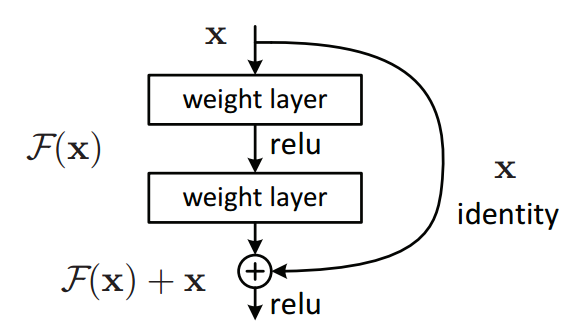
\includegraphics[width=200px]{residual_block.png}
	\caption{A residual block, figure taken from ref. \cite{resnet}}
	\label{fig:residual_block}
\end{figure}

A regular deep net can then be converted to a residual net by simply replacing stacks of convolutional layers by residual blocks. This turns out to work so well that the authors obtained first place in the 2015 ILSVRC classification competition, using an ensemble consisting of six 152-layer residual nets. 


\section{Methods}

\subsection{Data generation}
Our desired dataset consists of a set of sample states of the XY model on a square lattice of dimension $L$, each at fixed energy and temperature. As these are one to one only in the thermodynamic limit, we pick our representative states as those with approximately energy $E = \langle E \rangle$. Sampling the microcanonical ensemble quickly becomes unfeasible, and so we resort to sampling using a Markov-Chain Monte-Carlo(MCMC) method - the Metropolis algorithm. To generate a state at temperature T, we start with a uniformly distributed spin configuration. We then run the Metropolis algorithm(shown below) until successive energy values are within a specified tolerance, at which point we assume equilibrium has been reached. For calculating expectation values - energy in particular - we then proceed to sample the state space $M = 1000$ times, each separated by $5L^2$ Metropolis steps to minimize autocorrelations in the states.

\begin{algorithm}
	\caption{The Metropolis algorithm. Above we illustrate a full sweep, e.g. an MCMC step applied to each spin in the system.}
	
	T = get\_temperature()\\
	set\_initial\_config()\\
	$E_0$ = energy()\\

	\For{\text{s in spins}}{
		flip\_spin(s)\\
		$E_1$ = compute\_energy()\\
		$\Delta E$ = $E_1 - E_0$\\
		acc = uniform\_random()\\
		\If{\text{acc} $ < \exp\left(-\Delta E/T\right)$}{
			Update current state, store\\
			$C_0 = C_1$\\
			$E_0 = E_1$\\
		}
	}
\end{algorithm} 
\vspace{5px}

INDICATION: (170,70) ETA = 0.0001
https://arxiv.org/pdf/1207.0580.pdf Hinton paper
https://machinelearningmastery.com/machine-learning-ensembles-with-r/

\section{Results}
We begin by reporting on the quality of our generated datasets. It's a mixed bag - while all datasets generate the expected energy and heat capacity curves(see Fig. \ref{fig:energy_heatcap_example}), we can determine that the statistical averages cannot be exactly correct. To do so, we refer to the fact that one may determine the scaling of $T_\text{KT}$ with lattice dimension $L$ with the help of renormalization group techniques. In particular, the scaling is given by\cite{PhysRevLett.39.1201}
\begin{align}
T_\text{KT}^L = T_\text{KT}^\infty + c\frac{1}{(\log L)^2}
\end{align}
where $c$ is a constant. This is unfortunately not the scaling we see, as shown in Fig. \ref{fig:tkt_scaling_L}. Nonetheless, each dataset \textit{does} have a well-defined transition temperature, as may be observed by the maximum in the heat capacity. And we can still see whether our neural nets can learn this particular point if we feed them either the spin or vortex configuration.

\subsection{Convolutional nets}
In order to obtain the best possible fit, we have tried out several architectures.\footnote{Calling them architectures might be a little excessive; various orderings of various layers might be more appropriate!} We begin by looking at our results on the simplest possible CNN



\bibliographystyle{unsrt}
\bibliography{bib}

\end{document}